%%%%%%%%%%%%%%%%%%%%%%%%%%%%%%%%%%%%%%%%%%%%%%%%%%%%%%%%%%%
%--------------------------------------------------------
%  ____  _           
% |  _ \| |__   ___  
% | |_) | '_ \ / _ \ 
% |  _ <| | | | (_) |
% |_| \_\_| |_|\___/ 
%
% LaTeX2e Template - Modified for UI Stochastic Modeling Project
% --------------------------------------------------------
%%%%%%%%%%%%%%%%%%%%%%%%%%%%%%%%%%%%%%%%%%%%%%%%%%%%%%%%%%%

\documentclass[9pt,a4paper,twocolumn,twoside]{rho-class/rho}
\usepackage[english]{babel} % Menggunakan Bahasa Inggris

% Menambahkan paket listings untuk optimasi compile-time
\usepackage{listings}
\usepackage{xcolor}
\usepackage{url}

% Konfigurasi warna kode R
\definecolor{codegreen}{rgb}{0,0.6,0}
\definecolor{codegray}{rgb}{0.5,0.5,0.5}
\definecolor{codepurple}{rgb}{0.58,0,0.82}
\definecolor{backcolour}{rgb}{0.95,0.95,0.92}

\lstset{
    backgroundcolor=\color{backcolour},   
    commentstyle=\color{codegreen},
    keywordstyle=\color{magenta},
    numberstyle=\tiny\color{codegray},
    stringstyle=\color{codepurple},
    basicstyle=\ttfamily\footnotesize,
    breakatwhitespace=false,         
    breaklines=true,                 
    captionpos=b,                    
    keepspaces=true,                 
    numbers=left,                    
    numbersep=5pt,                  
    showspaces=false,                
    showstringspaces=false,
    showtabs=false,                  
    tabsize=2,
    language=R
}

%----------------------------------------------------------
% Title
%----------------------------------------------------------
\doctype{Research Article}
\title{Multi-State Modeling After Bone Marrow Transplantation: A Continuous-Time Markov Chain Approach}

%----------------------------------------------------------
% Authors, Affiliations and dates
%----------------------------------------------------------
\author[{\textasteriskcentered},a,1]{Muhammad Zaki Zulhamlizar}
\author[{\textdagger},a,2]{Louisa Devina}
\author[{\textdagger},a,3]{Andhika Dzaky Karafathi}
\author[{\textdagger},a,4]{Muhammad Salman} 

\affil[a]{Department of Mathematics, Faculty of Mathematics and Natural Sciences, Universitas Indonesia, Depok, Indonesia}

%----------------------------------------------------------
% Corresponding author- information
%----------------------------------------------------------
\corres{\textsuperscript{\textasteriskcentered}Corresponding author: \href{mailto:zaki.zulhamlizar@sci.ui.ac.id}{zaki.zulhamlizar@sci.ui.ac.id}}
\corres{\textsuperscript{\textdagger}These authors contributed equally to this work.}

\docinfo{Final Project Model Stokastik 1. Submitted on June 12, 2026, via EMAS3.} 

\journalname{Universitas Indonesia}
\journal{Stochastic Models 1 Project}
\theday{\today}
\vol{2026}
\no{1}

%----------------------------------------------------------
% Abstract and Keywords
%----------------------------------------------------------
\begin{abstract}
    This study implements a time-homogeneous Continuous-Time Markov Chain (CTMC) framework to model the longitudinal clinical pathways of patients following allogeneic bone marrow transplantation (BMT). Utilizing the \texttt{ebmt4} registry comprising 2,279 leukemia patients from the \texttt{mstate} package in \texttt{R}, we construct a 6-state multi-state topology encompassing four transient phases (Transplant, Recovery, Adverse Event, and Combined Rec+AE) and two competing absorbing states (Relapse and Death). Transition intensities for the infinitesimal generator matrix $\mathbf{Q}$ are estimated via parametric Maximum Likelihood Estimation (MLE), and macro-level cohort trajectories are resolved across short-term, one-year, and asymptotic landmarks using matrix exponential evaluations $\exp(\mathbf{Q}t)$. Empirical results indicate that the baseline leaving rate from the initial transplant state yields an expected sojourn time of 467.92 days, with a slightly higher initial intensity toward complications ($q_{13}=0.000996$) over pure recovery ($q_{12}=0.000862$). Asymptotically ($t \to \infty$), the system converges to an ultimate terminal absorption allocation of 44.14\% for Relapse and 55.86\% for Death. Compared to conventional univariate survival curves, this multi-state approach provides significantly higher prognostic differentiation by successfully capturing risk trajectories within intermediate transient states without informational loss due to non-informative censoring.
\end{abstract}

\keywords{Continuous-Time Markov Chain, Multi-State Models, Infinitesimal Generator Matrix, Matrix Exponential, Bone Marrow Transplantation}

%----------------------------------------------------------
\begin{document}

    \maketitle
    \thispagestyle{firststyle}

%----------------------------------------------------------
% SECTION 1: PENDAHULUAN
%----------------------------------------------------------
\section{Introduction}
    \rhostart{H}ematological malignancies, particularly leukemia, continue to pose a substantial global health and economic burden, demanding aggressive and sophisticated therapeutic interventions \cite{Sung2021}. While the clinical maturation of allogeneic bone marrow transplantation (BMT) has fundamentally revolutionized leukemia treatment protocols \cite{Thomas1975, Copelan1991}, the post-transplantation recovery trajectory is rarely linear and is heavily characterized by highly dynamic intermediate clinical phases. Patients do not simply transition from health to death; instead, they navigate a complex network of interleaved physiological events, such as graft-versus-host disease (GvHD), delayed platelet recovery, and the perpetual threat of disease recurrence based on clinical registry guidelines \cite{EBMT2024}. These clinical phases do not occur in isolation but function as a series of time-dependent competing risks, making the accurate prognostic tracking of post-BMT cohorts a critical necessity in modern biostatistics, mathematical statistics, and actuarial science \cite{Charpentier2014, BlierWong2024, Putter2007, gsoutinhoebmt4}.

    Conventional survival analysis techniques, such as the classical Kaplan-Meier product-limit estimator and the Cox proportional hazards model, possess fundamental structural limitations when handling these multidirectional clinical pathways \cite{KleinMoeschberger2003}. Because traditional frameworks are inherently bivariate, they are strictly restricted to modeling a single, binary transition from an initial state to a single terminal endpoint, thereby rendering them inadequate for branching multi-state systems. To resolve this methodological constraint, multi-state modeling via a Continuous-Time Markov Chain (CTMC) framework is adopted \cite{AndersenKeiding2002, vanhouwelingen2012dynamic}. This stochastic framework explicitly maps the longitudinal trajectory of individuals through a finite discrete state space over continuous time \cite{Norris1997}. By utilizing an infinitesimal generator matrix $\mathbf{Q}$ to capture localized transition intensities, the system leverages the Kolmogorov forward differential equations to resolve macro-level transient state occupancy probabilities over time \cite{CoxMiller1965, fiocco2008reduced}.

    Although advanced multi-state techniques have become a standard benchmark internationally for evaluating clinical registries \cite{dewreede2011mstate}, their rigorous application within academic research in Indonesia remains markedly sparse, with the majority of domestic epidemiological literature still bound to conventional univariate models \cite{KemenKes2023}. This study directly bridges this methodological gap by systematically executing a time-homogeneous CTMC analysis on the comprehensive \texttt{ebmt4} blood and marrow transplantation dataset, consisting of 2,279 leukemia patients \cite{deWreede2010}. By enforcing an explicit constant intensity constraint, this paper provides a robust first-order approximation of the system \cite{KalbfleischLawless1985}, unlocking precise, interpretable metrics including expected clinical sojourn times and long-term asymptotic absorption allocations that enhance the prognostic utility of standard medical data.

    \subsection{Problem Formulation}
    Based on the outlined background and structural constraints of the clinical registry, this research formulates the following problems:
    \begin{enumerate}
        \item How to construct a mathematical 6-state transition architecture that accurately enscapulates the dynamic, interleaved clinical trajectories of leukemia patients post-BMT?
            
        \item How to estimate the constant transition intensities of the infinitesimal generator matrix $\mathbf{Q}$ using parametric Maximum Likelihood Estimation (MLE) under a time-homogeneous assumption?
        
        \item To what extent does the time-homogeneous CTMC framework unlock advanced prognostic indicators—specifically explicit milestone probability matrices, expected sojourn times, and asymptotic absorption allocations—compared to conventional bivariate survival approaches?
    \end{enumerate}
        
    \subsection{Research Objectives}
    The primary objectives of this research are defined as follows:
    \begin{enumerate}
        \item To design a unidirectional 6-state transition graph and restructure the comprehensive longitudinal data into an exposure-at-risk long format compatible with multi-state processing.
            
        \item To estimate the complete infinitesimal generator matrix $\mathbf{Q}$ by evaluating empirical transition events against cumulative person-days exposure via parametric maximum likelihood estimators.
        
        \item To compute and interpret short-term milestones, theoretical continuous time spent inside each clinical compartment, and the final competing risk distributions at the true asymptotic limit.
    \end{enumerate}
        
    \subsection{Significance and Benefits}
    This research provides substantial insights across both theoretical and practical dimensions:
    \begin{itemize}
        \item Theoretical Contributions: This study enriches the domestic statistical literature in Indonesia by providing a rigorous, reproducible documentation of parametric CTMC workflows applied to complex biomedical datasets, effectively bridges pure Markovian transition theory with applied multi-state biostatistics.
        
        \item Practical Applications: The calibrated model delivers intuitive, data-driven prognostic matrices and trajectory visualizations capable of supporting clinical epidemiologists in therapeutic decision-making. Furthermore, the established computational pipeline can be readily adapted to evaluate other multi-phase chronic conditions, such as cardiovascular diseases or oncology registries.
    \end{itemize}
        
    \subsection{Scope and Limitations}
    To preserve analytical focus and maintain mathematical consistency, the boundaries of this study are restricted to the following parameters:
    \begin{itemize}
        \item Data Source Constraints: The analysis is strictly secondary, utilizing the historical \texttt{ebmt4} bone marrow transplantation registry available within the \texttt{mstate} package, which encapsulates the longitudinal records of 2,279 leukemia patients \cite{dewreede2011mstate}. No primary field data collection was conducted.
        
        \item Time-Homogeneity Assumption: The model operates under a strict time-homogeneous constraint where transition intensities are assumed constant over time. While true biological hazards are inherently non-homogeneous, this assumption is enforced as a foundational first-order mathematical approximation.
        
        \item Parametric Methodological Focus: Parameter calibration is restricted to parametric Maximum Likelihood Estimation (MLE) for the generator matrix and direct matrix exponential evaluations $\exp(\mathbf{Q}t)$ for transient projections. Non-parametric extensions and semi-parametric regression structures utilizing patient-specific covariates are outside the scope of this study.
        
        \item Transition Graph Architecture: The state space is bounded by a 6-state multi-state topology, consisting of four transient phases (\textit{Transplant, Recovery, Adverse Event, and Combined Rec+AE}) and two competing terminal absorbing destinations (\textit{Relapse and Deceased}). Alternative branching paths or re-entry geometries are not explored.
    \end{itemize}

%----------------------------------------------------------
% SECTION 2: METHODOLOGY
%----------------------------------------------------------
\section{Methodology}

    This section outlines the mathematical framework of the multi-state model using a continuous-time stochastic approach. The state space configuration, parameter estimation via maximum likelihood, and long-term limiting behaviors are defined to establish the analytical framework.

    \subsection{Model Description}
        To model the longitudinal transitions of individuals across distinct clinical phases, a Continuous-Time Markov Chain (CTMC) framework is utilized \cite{Norris1997, Dobrow2016}. Let $\{X(t), t \geq 0\}$ be a continuous-time stochastic process taking values in a finite state space $\mathcal{S} = \{1, 2, \dots, K\}$. The process satisfies the Markov property for a time-homogeneous process, meaning that for any states $i, j \in \mathcal{S}$ and time points $0 \leq s \leq t$, the conditional probability distribution of any future state depends strictly on the current state:

        \begin{equation}
            P(X(t) = j \mid X(s) = i, \{X(u) : 0 \leq u < s\}) = P(X(t) = j \mid X(s) = i)
        \end{equation}
        
        The time-homogeneous assumption states that transition intensities depend strictly on the elapsed time between states rather than the absolute historical timeline, serving as an analytical baseline for evaluating transition behavior \cite{CoxMiller1965}.

    \subsection{State Space and Transition Architecture}
        The structural architecture is configured as an interleaved 6-state multi-state system, preserving the natural clinical evolution of individuals post-intervention. The finite state space is defined as $\mathcal{S} = \{1, 2, 3, 4, 5, 6\}$, representing:
        \begin{itemize}
            \item State 1 (Tx): Initial baseline state (Initial entry).
            \item State 2 (Rec): Intermediate transient recovery state.
            \item State 3 (AE): Intermediate transient adverse event state.
            \item State 4 (Rec+AE): Combined dual-transient intermediate state.
            \item State 5 (Rel): Competing absorbing state (Treatment failure via relapse).
            \item State 6 (Death): Competing absorbing state (Terminal failure).
        \end{itemize}
        The permissible instantaneous paths within this system are mathematically restricted. States 5 and 6 are strictly designated as absorbing states, meaning that once the process enters these states, the leaving rate is identically zero ($q_{5j} = q_{6j} = 0, \forall j \in \mathcal{S}$) \cite{AndersenKeiding2002}.

    \subsection{Mathematical Formulation and Intensity Estimation}
        The transition behavior of the CTMC is governed by the infinitesimal generator matrix, denoted as $\mathbf{Q} \in \mathbb{R}^{K \times K}$ \cite{Norris1997}. The off-diagonal elements $q_{ij}$ (where $i \neq j$) represent the instantaneous transition intensities from state $i$ to state $j$, formulated as:

        \begin{equation}
            q_{ij} = \lim_{\Delta t \to 0} \frac{P(X(t + \Delta t) = j \mid X(t) = i)}{\Delta t}
        \end{equation}

        The diagonal elements $q_{ii}$ represent the total rate of leaving state $i$ and are constrained by the conservation law, forcing the rows of the generator matrix to sum to zero \cite{CoxMiller1965}:

        \begin{equation}
            q_{ii} = - v_i = - \sum_{j \neq i} q_{ij}
        \end{equation}

        The parameters of the generator matrix are estimated using parametric Maximum Likelihood Estimation (MLE) under continuous observation \cite{KalbfleischLawless1985}. Let $D_{ij}$ denote the total number of observed transitions from state $i$ to state $j$ across the sample. Let $E_i$ represent the cumulative total time-at-risk (total exposure time) that individuals spent inside state $i$ prior to transitioning or censoring. The constant intensity estimator is given by:

        \begin{equation}
            \hat{q}_{ij} = \frac{D_{ij}}{E_i} = \frac{D_{ij}}{\sum_{m} (T_{\text{stop}, m}^{(i)} - T_{\text{start}, m}^{(i)})}
        \end{equation}

    \subsection{Transient Probabilities and Limiting Behavior}
        The state probabilities of the system are governed by the transition probability function matrix, $\mathbf{P}(t) \in \mathbb{R}^{K \times K}$, where each entry $P_{ij}(t) = P(X(t) = j \mid X(0) = i)$. The evolution of $\mathbf{P}(t)$ satisfies the system of differential equations described by the Kolmogorov Forward Equations \cite{CoxMiller1965}:

        \begin{equation}
            \frac{d}{dt}\mathbf{P}(t) = \mathbf{P}(t)\mathbf{Q}
        \end{equation}
        
        Under the time-homogeneous assumption, the explicit solution to this system for any duration $t$ is computed via the matrix exponential:
        
        \begin{equation}
            \mathbf{P}(t) = \exp(\mathbf{Q}t) = \sum_{k=0}^{\infty} \frac{(\mathbf{Q}t)^k}{k!}
        \end{equation}
        
        The asymptotic characteristics of the system are evaluated by computing the limiting distribution as $t$ approaches infinity. For systems containing absorbing states, the limiting probability matrix captures the ultimate absorption allocation \cite{Norris1997}:

        \begin{equation}
            \mathbf{P}_{\infty} = \lim_{t \to \infty} \exp(\mathbf{Q}t)
        \end{equation}

    \subsection{Sojourn Time Distribution}
        The continuous duration within each transient state is evaluated through the concept of sojourn times. In a time-homogeneous CTMC, the random variable $S_i$, representing the continuous time an individual resides in a transient state $i$ before transitioning, follows an Exponential distribution parametrized by the leaving rate $v_i = -q_{ii}$ \cite{Norris1997}:

        \begin{equation}
            S_i \sim \text{Exponential}(v_i)
        \end{equation}

        Consequently, the expected sojourn time spent inside a specific compartment $i$ is defined as the inverse of its leaving hazard:

        \begin{equation}
            \mathbb{E}[S_i] = \frac{1}{v_i} = \frac{1}{-q_{ii}}
        \end{equation}

        For absorbing states where $q_{ii} = 0$, the expected sojourn time resolves to infinity ($\infty$), representing the mathematical property of an absorbing state.

    \subsection{Computational Implementation and Software}
        Data processing and numerical computations are executed within the \texttt{R} statistical programming environment. Longitudinal data preparation, specifically the conversion from wide-format records to multi-state long-format exposures, is performed via the \texttt{msprep} function from the \texttt{mstate} package \cite{dewreede2011mstate}. 
        
        The numerical solution for the matrix exponential $\exp(\mathbf{Q}t)$ is evaluated using the \texttt{expm} algorithm provided by the \texttt{Matrix} package. Longitudinal trajectories and state probability functions are constructed and exported utilizing the \texttt{tidyverse} architecture and \texttt{ggplot2} visualization libraries. The complete, reproducible computational pipeline and LaTeX source codes are publicly available at \url{https://github.com/zakizulham/Multi-State-Modeling-After-Bone-Marrow-Transplantation}.

%----------------------------------------------------------
% SECTION 3: HASIL DAN PEMBAHASAN
%----------------------------------------------------------
\section{Results and Discussion}
    This section presents the empirical outputs, structural estimations, and long-term prognostic trajectories derived from the multi-state calibration of the \texttt{ebmt4} cohort data.

    \subsection{Presentation of Results}
        The multi-state transformation of the longitudinal registry mapped a total of 12 active clinical transition pathways across 2,279 patients. Table~\ref{tab:transition_rates} summarizes the empirical event counts and total time-at-risk exposures (expressed in person-days) that serve as the mathematical foundation for the maximum likelihood estimation of the daily transition intensities ($q_{ij}$).

        \begin{table}[H]
        \centering
        \caption{Empirical Transition Events and Exposures for the 6-State Model}
        \label{tab:transition_rates}
        \resizebox{\columnwidth}{!}{
        \begin{tabular}{ccccc}
        \hline
        From State ($i$) & To State ($j$) & Total Events & Total Exposure (Days) & Intensity Rate ($q_{ij}$) \\
        \hline
        Tx     & Rec    & 785 & 911,046   & 0.000862 \\
        Tx     & AE     & 907 & 911,046   & 0.000996 \\
        Tx     & Rel    & 95  & 911,046   & 0.000104 \\
        Tx     & Death  & 160 & 911,046   & 0.000176 \\
        Rec    & Rec+AE & 227 & 977,570   & 0.000232 \\
        Rec    & Rel    & 112 & 977,570   & 0.000115 \\
        Rec    & Death  & 39  & 977,570   & 0.000040 \\
        AE     & Rec+AE & 433 & 765,784   & 0.000565 \\
        AE     & Rel    & 56  & 765,784   & 0.000073 \\
        AE     & Death  & 197 & 765,784   & 0.000257 \\
        Rec+AE & Rel    & 107 & 1,077,153 & 0.000099 \\
        Rec+AE & Death  & 137 & 1,077,153 & 0.000127 \\
        \hline
        \end{tabular}
        }
        \end{table}

        These estimated hazards establish the off-diagonal parameters of the infinitesimal generator matrix $\mathbf{Q}$. Enforcing the row-stochastic conservation law yields the complete $6 \times 6$ operator structured as follows:
        
        \begin{equation}
        \small
        \mathbf{Q}=
        \scalebox{0.78}{$
        \begin{pmatrix}
        -0.002137 & 0.000862 & 0.000996 & 0.000000 & 0.000104 & 0.000176\\
         0.000000 & -0.000387 & 0.000000 & 0.000232 & 0.000115 & 0.000040\\
         0.000000 & 0.000000 & -0.000896 & 0.000565 & 0.000073 & 0.000257\\
         0.000000 & 0.000000 & 0.000000 & -0.000227 & 0.000099 & 0.000127\\
         0.000000 & 0.000000 & 0.000000 & 0.000000 & 0.000000 & 0.000000\\
         0.000000 & 0.000000 & 0.000000 & 0.000000 & 0.000000 & 0.000000
        \end{pmatrix}
        $}
        \end{equation}

        Evaluating the negative inverse of the main diagonal elements yields the expected clinical sojourn times spent inside each compartment before a patient transfers out, as tabulated in Table~\ref{tab:sojourn_times}.
        \begin{table}[H]
        \centering
        \caption{Expected Sojourn Times Across Transient Clinical States}
        \label{tab:sojourn_times}
        \resizebox{0.9\columnwidth}{!}{
        \begin{tabular}{lcc}
        \hline
        Clinical State & Leaving Rate ($v_i$) & Expected Sojourn (Days) \\
        \hline
        Tx     & 0.002137 & 467.92 \\
        Rec    & 0.000387 & 2586.16 \\
        AE     & 0.000896 & 1116.30 \\
        Rec+AE & 0.000227 & 4414.56 \\
        Rel    & 0.000000 & $\infty$ (Absorbing State) \\
        Death  & 0.000000 & $\infty$ (Absorbing State) \\
        \hline
        \end{tabular}
        }
        \end{table}

        To map macro-level clinical progressions, the transient transition probability matrices $\mathbf{P}(t)$ were resolved via matrix exponential operations. At the short-term clinical landmark ($t = 100$ days), the matrix $\mathbf{P}(100)$ is given by:

        \begin{equation}
        \small
        \setlength{\arraycolsep}{2.2pt}
        \mathbf{P}(100)=
        \begin{pmatrix}
        0.8076 & 0.0760 & 0.0856 & 0.0034 & 0.0102 & 0.0171\\
        0.0000 & 0.9621 & 0.0000 & 0.0225 & 0.0114 & 0.0041\\
        0.0000 & 0.0000 & 0.9143 & 0.0535 & 0.0073 & 0.0250\\
        0.0000 & 0.0000 & 0.0000 & 0.9776 & 0.0098 & 0.0126\\
        0.0000 & 0.0000 & 0.0000 & 0.0000 & 1.0000 & 0.0000\\
        0.0000 & 0.0000 & 0.0000 & 0.0000 & 0.0000 & 1.0000
        \end{pmatrix}
        \end{equation}

        At the one-year clinical landmark ($t = 365$ days), capturing long-term patient dynamics, the operational matrix $\mathbf{P}(365)$ resolves to:

        \begin{equation}
        \small
        \setlength{\arraycolsep}{2.2pt}
        \mathbf{P}(365)=
        \begin{pmatrix}
        0.4584 & 0.2018 & 0.2107 & 0.0351 & 0.0352 & 0.0588\\
        0.0000 & 0.8684 & 0.0000 & 0.0758 & 0.0404 & 0.0154\\
        0.0000 & 0.0000 & 0.7211 & 0.1686 & 0.0260 & 0.0843\\
        0.0000 & 0.0000 & 0.0000 & 0.9206 & 0.0348 & 0.0446\\
        0.0000 & 0.0000 & 0.0000 & 0.0000 & 1.0000 & 0.0000\\
        0.0000 & 0.0000 & 0.0000 & 0.0000 & 0.0000 & 1.0000
        \end{pmatrix}
        \end{equation}

        Finally, the asymptotic limiting behavior of the multi-state system as $t \to \infty$ evaluates the true terminal absorption matrix, settling the ultimate competing risk distribution:

        \begin{equation}
        \small
        \setlength{\arraycolsep}{2.2pt}
        \mathbf{P}(\infty)=
        \begin{pmatrix}
        0.00000 & 0.00000 & 0.00000 & 0.00000 & 0.44140 & 0.55860\\
        0.00000 & 0.00000 & 0.00000 & 0.00000 & 0.55964 & 0.44036\\
        0.00000 & 0.00000 & 0.00000 & 0.00000 & 0.35843 & 0.64157\\
        0.00000 & 0.00000 & 0.00000 & 0.00000 & 0.43852 & 0.56148\\
        0.00000 & 0.00000 & 0.00000 & 0.00000 & 1.00000 & 0.00000\\
        0.00000 & 0.00000 & 0.00000 & 0.00000 & 0.00000 & 1.00000
        \end{pmatrix}
        \end{equation}
        
    \subsection{Interpretation}
        The empirical parameters computed from the 6-state CTMC framework offer granular insights into post-transplantation kinetics, translating abstract transition intensities into concrete clinical prognosis.

        \subsubsection{Analysis of Intensities and Sojourn Times}
            The estimated infinitesimal generator matrix indicates that patients in the initial transplantation state (\texttt{Tx}) exhibit a higher instantaneous tendency to transition directly toward the Adverse Event phase (\texttt{AE}, $q_{13}=0.000996$) than toward pure Recovery (\texttt{Rec}, $q_{12}=0.000862$). Direct terminal transitions from baseline to Relapse ($q_{15}=0.000104$) or Death ($q_{16}=0.000176$) remain minimal, confirming that post-BMT failure routes operate predominantly through intermediate transient pathways. 

            The baseline leaving rate ($v_1=0.002137$) translates into an expected sojourn time of $467.92$ days, indicating that patients spend a considerable duration in the primary post-graft phase before developing distinct physiological paths. Within the intermediate transient compartments, the pure Recovery phase (\texttt{Rec}) manifests a substantial expected sojourn of $2,586.16$ days, with its dominant exit path targeting the compound \texttt{Rec+AE} state ($q_{24}=0.000232$). This highlights that even after establishing hematological recovery, patients remain highly exposed to delayed post-transplant complications. 

            For the acute Adverse Event phase (\texttt{AE}), the propensity to progress into the compound history state \texttt{Rec+AE} ($q_{34}=0.000565$) is significantly higher than immediate failure rates ($q_{35}=0.000073$, $q_{36}=0.000257$), outlining a clinical buffer zone where acute toxicities frequently overlap with late-stage recoveries. Notably, the compound \texttt{Rec+AE} state exhibits an elevated theoretical sojourn time of $4,414.56$ days. Once transitions eventually activate from this dual-history state, the daily hazard of mortality ($q_{46}=0.000127$) systematically dominates over disease relapse ($q_{45}=0.000099$), pointing to non-relapse mortality driven by cumulative physiological stress as the primary risk.

        \subsubsection{Evolution of Transition Probabilities}
            Evaluating the matrix exponential at specific time landmarks isolates the macro-level distribution of the patient cohort across various longitudinal stages.
            \begin{itemize}
                \item Short-Term Milestone ($t=100$ days): At 100 days post-transplantation, a patient entering at \texttt{Tx} retains an $80.76\%$ probability of occupying the initial baseline condition. The immediate short-term occupancy for pure Recovery and Adverse Events stands at $7.60\%$ and $8.56\%$ respectively, while early terminal failure remains suppressed ($\text{Rel}=1.02\%$, $\text{Death}=1.71\%$). This mathematically proves that major multi-state differentiation occurs post-landmark.
                
                \item One-Year Milestone ($t=365$ days): After one year, the baseline probability drops substantially to $45.84\%$. Simultaneously, the probability mass shifts toward active intermediate transient states, with \texttt{Rec} and \texttt{AE} climbing to $20.18\%$ and $21.07\%$ respectively. Cumulative mortality reaches $5.88\%$, surpassing relapse occupancy ($3.52\%$), indicating a steady, gradual structural progression.
                
                \item Asymptotic Limiting Behavior ($t\rightarrow\infty$): At the true asymptotic limit, all transient occupancy probabilities converge to zero, and the cohort is fully absorbed by the two terminal sinks. For a baseline patient (\texttt{Tx}), the final distribution converges to a $44.14\%$ probability of ultimate absorption into \texttt{Relapse} and a dominant $55.86\%$ probability of absorption into \texttt{Death}, resolving the definitive long-term competing risk layout.
            \end{itemize}

            The continuous trajectory of these evolving state occupancy functions is visually mapped across a 2,000-day tracking horizon in Figure~\ref{fig:long-term probability}, demonstrating the rapid exhaustion of the baseline phase, the transient peaking of intermediate stages, and the monotonic growth of competing absorbing endpoints.

            \begin{figure}[t!]
            \centering
            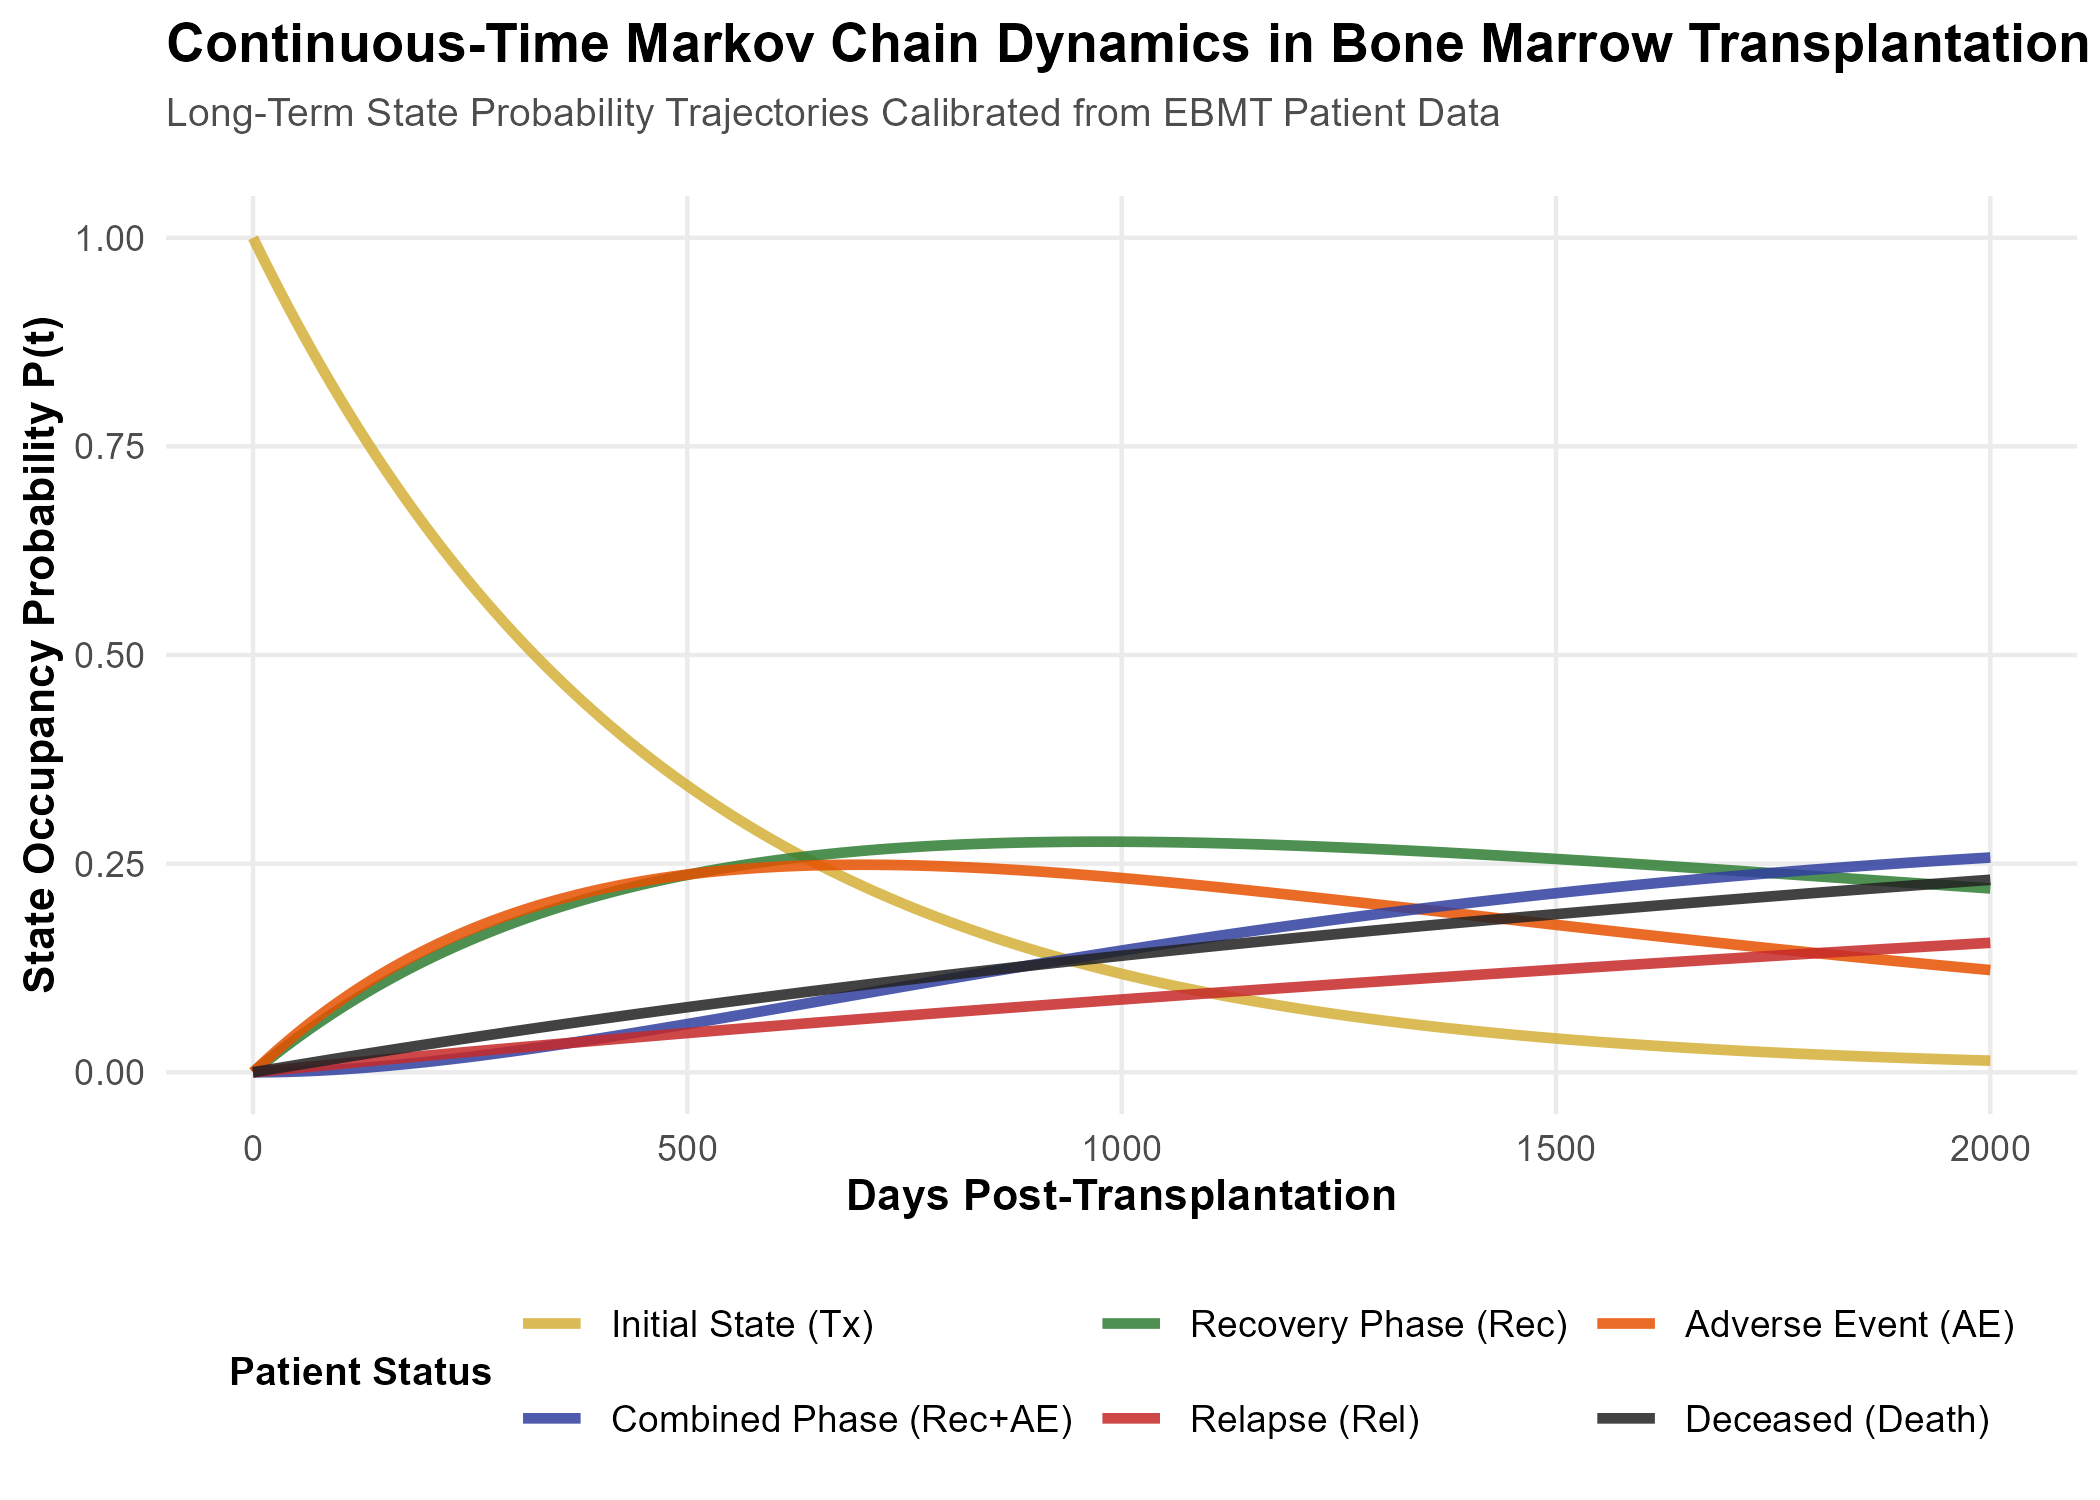
\includegraphics[width=\columnwidth]{figures/ctmc_trajectory.png}
            \caption{Continuous-Time Markov Chain State Probability Trajectories over 2,000 Days.}
            \label{fig:long-term probability}
            \end{figure}
        
    \subsection{Comparison and Validation}
        The 6-state CTMC framework provides higher analytical granularity compared to standard non-parametric survival tools like the Kaplan-Meier product-limit estimator. Traditional survival curves are mathematically restricted to single-event layouts, tracking cohorts from baseline exclusively to a binary endpoint (overall survival). In such rigid architectures, critical intermediate multi-state trajectories—such as recovering blood counts or suffering acute toxicities—are either completely missed or treated as non-informative right-censoring, which simplifies the longitudinal clinical timeline.

        In contrast, the implemented CTMC model validates its prognostic power by simultaneously tracking interlocking intermediate paths and terminal endpoints via $\mathbf{P}(t)=\exp(\mathbf{Q}t)$. For instance, at the one-year mark, a standard Kaplan-Meier curve would only report a blanket survival rate. The multi-state model, however, dissects this survival mass into precise components: proving that $45.84\%$ remain stable at baseline, while $20.18\%$ and $21.07\%$ are currently battling localized recovery and complication states respectively. 

        Furthermore, the limiting distribution $\mathbf{P}(\infty)$ uncovers an essential clinical phenomenon. Patients who successfully transition into the pure Recovery phase (\texttt{Rec}) display a higher final probability of absorbing into Relapse ($55.96\%$) because they survived early procedural mortality risks. Conversely, falling into an Adverse Event (\texttt{AE}) increases the final probability of absorption into Deceased ($64.16\%$), providing a mathematical validation of transplant-related toxicities driving non-relapse mortality. This deep prognostic layer, illustrating how past transient status influences final terminal risks, cannot be directly extracted via conventional bivariate survival curves.
        
    \subsection{Strengths and Limitations}
      The primary strength of this 6-state configuration is its capacity to map multidirectional post-BMT trajectories through 12 distinct transition pathways, including a compound history state (\texttt{Rec+AE}). This framework provides explicit continuous-time occupancy probabilities and expected sojourn durations, offering higher prognostic granularity than standard bivariate survival models.

      However, the model operates under three constraints. First, the time-homogeneous assumption treats transition intensities as constant, whereas biological hazards typically fluctuate over time. Second, the first-order Markov property enforces memorylessness, ignoring the actual duration a patient previously spent in prior states. Finally, the boundaries are data-restricted by the \texttt{ebmt4} registry, which treats Relapse as a terminal absorbing state and precludes the evaluation of post-relapse mortality.

%----------------------------------------------------------
% SECTION 4: KESIMPULAN
%----------------------------------------------------------
\section{Conclusion}
    
    \subsection{Summary of Findings}
        This study demonstrated the implementation of a 6-state time-homogeneous Continuous-Time Markov Chain (CTMC) model on the \texttt{ebmt4} dataset ($2,279$ patients) to evaluate longitudinal transitions across transient (\texttt{Tx}, \texttt{Rec}, \texttt{AE}, \texttt{Rec+AE}) and competing absorbing states (\texttt{Rel}, \texttt{Death}). Based on the calibrated generator matrix $\mathbf{Q}$ and matrix exponentials $\exp(\mathbf{Q}t)$, four core empirical insights are established:

        \noindent (1) Initial-phase hazard profiles: In the \texttt{Tx} state, the transition intensity toward Adverse Events ($q_{13} = 0.000996/\text{day}$) exceeded that toward Platelet Recovery ($q_{12} = 0.000862/\text{day}$), indicating a higher early susceptibility to complications than to recovery, with an expected baseline sojourn time of $467.92$ days. 

        \noindent (2) Sojourn time distribution parameters: Among the transient phases, the combined \texttt{Rec+AE} state exhibited the longest expected sojourn ($4,414.56$ days), followed by \texttt{Rec} ($2,586.16$ days) and \texttt{AE} ($1,116.30$ days). In the \texttt{Rec+AE} compartment, mortality constituted the dominant risk as the daily hazard of Death ($q_{46} = 0.000127$) systematically exceeded Relapse ($q_{45} = 0.000099$).

        \noindent (3) Time-specific probability landmarks: At 100 days post-BMT, $80.76\%$ of patients starting in \texttt{Tx} remained in the initial baseline condition. By 365 days, this occupancy dropped to $45.84\%$, while \texttt{Rec} and \texttt{AE} states rose to $20.18\%$ and $21.07\%$ respectively, confirming a gradual structural transition layout. 
        
        \noindent (4) Asymptotic long-run absorption: As $t \to \infty$, the state dynamics for a baseline patient (\texttt{Tx}) converge to an ultimate terminal absorption allocation of $44.14\%$ for \texttt{Relapse} and $55.86\%$ for \texttt{Death}. 

        Collectively, these multi-state parameters provide a statistically consistent and clinically relevant representation of post-transplantation dynamics that cannot be captured by a standard Kaplan-Meier curve.
        
    \subsection{Implications}
        Methodologically, this work confirms the CTMC multi-state framework as a principled alternative to bivariate survival models. Calibrating 12 transition intensities simultaneously through the MLE estimator $D_{ij} / E_i$, and resolving the full probability trajectory through the matrix exponential $\exp(\mathbf{Q}t)$, avoids the information loss caused by treating intermediate clinical events as censored data points. The complete analytical workflow, from \texttt{msprep()} long-format conversion through matrix exponential computation via \texttt{expm} to \texttt{ggplot2} visualization, is structured to be reproducible and adaptable to similar longitudinal clinical registries.

        On the applied side, the baseline \texttt{Tx}-to-\texttt{AE} intensity exceeding the \texttt{Tx}-to-\texttt{Rec} intensity serves as a statistical indicator that clinical complications frequently precede stable recovery for a large portion of the cohort, warranting close monitoring in the early post-transplant window. The dominance of Death over Relapse as the final absorbing state, sitting at $55.86\%$ versus $44.14\%$ for a \texttt{Tx}-origin patient, further reinforces that clinical protocols focused on mortality prevention across all transient phases deserve equal or greater attention than relapse prevention alone. These are granular risk-differentiations that standard univariate survival curves cannot extract. 
        
    \subsection{Recommendations}
      Several methodological directions are proposed to extend the analytical utility of this framework. \textit{First,} the time-homogeneous assumption constrains the transition intensities $q_{ij}$ to remain constant. In clinical applications, these hazards typically exhibit time-dependent fluctuations, often peaking in the acute post-transplantation phase. Future research should examine time-inhomogeneous CTMC specifications or semi-Markov models to permit state-specific empirical holding time distributions outside the Exponential family.

      \textit{Second,} the first-order Markov property assumes future transition probabilities are independent of the historical duration spent in prior states. Incorporating covariate-stratified Cox proportional hazards extensions within the \texttt{mstate} framework—linking patient-level variables such as age, disease subtype, and conditioning regimen directly to the intensity estimates—would address this memoryless constraint and refine the estimation of the generator matrix $\mathbf{Q}$.

      \textit{Third,} the prognostic scope is bounded by the tracking limitations of the \texttt{ebmt4} dataset, which classifies Relapse as a terminal absorbing state alongside Death. This structural constraint precludes the evaluation of post-relapse mortality dynamics. Utilizing extended longitudinal registries with systematic post-recurrence tracking would enable the mathematical modeling of these subsequent transition pathways.

      \textit{Fourth,} future work should incorporate the non-parametric Aalen-Johansen estimator as an analytical complement to the maximum likelihood approach, resolving transition probabilities without enforcing time-homogeneity constraints. \textit{Finally,} executing formal Markov property verifications and calibrating this multi-state framework using primary Indonesian clinical data represent essential prerequisites before these stochastic outputs can be applied to inform localized therapeutic decisions.


%----------------------------------------------------------
% REFERENCES
%----------------------------------------------------------
\printbibliography
\end{document}